% Copyright (C) 2011 Thomas L. Kula
% All Rights Reserved
%
% See the file LICENSE for license terms.
\documentclass[12pt]{article}
\usepackage{graphicx}
\usepackage{rotating}
\usepackage{fix-cm}
\usepackage{multirow}
\setlength{\paperwidth}{5.5in}
\setlength{\paperheight}{8.5in}
\setlength{\textheight}{7.45in}
\setlength{\topmargin}{-1.0in}
\setlength{\oddsidemargin}{-0.5in}
\setlength{\evensidemargin}{-0.5in}
\setlength{\textwidth}{4.0in}
\setlength{\parindent}{0in}
\setlength{\parskip}{3mm}
\usepackage[print]{booklet} \nofiles
\source{\magstep0}{5.5in}{8.5in}
\target{\magstep0}{11in}{8.5in}
\setpdftargetpages
\pagestyle{empty}
\begin{document}


\begin{center}
{\fontsize{36}{48}\selectfont \textsc{Haiku a Day }} \\
Sixth Anniversary Issue
\end{center}

\vspace*{3.5cm}

{\fontsize{20}{40}\selectfont 

A gentle burble

A metal monster's tummy

Cleans my dirty clothes


}

\vspace*{5.0cm}
\begin{center}
{\large{Issue 73: July 2011}} \\[5mm]
{\fontsize{8}{8}\selectfont  \textsc{ St. Joshua Norton Press }} \\[1mm]
{\fontsize{6}{6}\selectfont Mathom House in Midtown \textbar The People's Republic of Ames }
\end{center}


\newpage

Six years down, eh? That's nearly thirty-seven thousand syllables, over two
thousand haikus, and untold numbers of times I've sat at a coffee shop or
at the laundromat putting together that month's issue of HAD. 

Last month was also a spectacular month. Aside from making it through another
birthday (if 30 is the new 21, then 33 is the new 24, but most 24 year olds
only wish they were as awesome as this) I had a great vacation driving out
and hanging out for six days in New York City. And, frankly, I've been bitten
by the bug (and not a bed bug --- I checked for those!) It's my goal to live
there by this time next year, and it awoke in me the gumption to actually
look for a new job. Is it a hairbrained scheme? Absolutely. But sometime
you gotta take the hairbrained schemes and see where they go....

Until next month, enjoy.



--- Thomas

http://kula.tproa.net/had/ \\
kula@tproa.net

Download this and previous HADs at the website, so you can
print out your own (DIY, yeah!) or if you want me to send
you one, send me your address, and maybe a stamp if you
are feeling nice. Or send me something you've made ---
trades always appreciated, postcards are nice too.

\vfill


1 July 2011

O Canada Day! \\
I celebrate with poutine \\
And Moxy Fruvous

\newpage

2 July 2011

Ten hours, and five \\
Driving, time in Grand Rapids \\
Hang out with zine friends

3 July 2011

Why two pounds of peas? \\
Why not use three pounds of peas? \\
That sounds good to me.

4 July 2011

Could the pea salad \\
Just not want to get eaten? \\
Damn food poisoning

5 July 2011

This day, sleepy haze \\
And no appetite, defined \\
It passes quickly

6 July 2011

That color is blue. \\
I don't care for fancy names, \\
That color is blue.

7 July 2011

Where are your headlights? \\
Cars coming at me should be \\
Very brightly lit.

8 July 2011

There, a blinkylight \\
Let's the world know something {\em is} \\
Does anyone see?

\newpage

9 July 2011

Craving some baked goods \\
I have an oatmeal muffin \\
Tasty and fiber

10 July 2011

I hate buying shoes \\
They never have what I want \\
This goes for clothes too

11 July 2011

A crack in the sky \\
Losing their bottoms, the clouds \\
Rain down upon us

12 July 2011

As I leave, mats come \\
Much work when I get back here \\
But now, conference

13 July 2011

A book warrior \\
Devoutly guards his building \\
No unknowns will pass

14 July 2011

Late walk, Central Park \\
City explodes above me \\
I am mesmerised

15 July 2011

Delta: Always late \\
Chillin' at Newark Airport \\
What more can I say?

\newpage

16 July 2011

Twelve hours of heat \\
Shadow Art Fair at Corner \\
Luckily there's beer

17 July 2011

Oversleep, Mom calls, \\
I get out of bed, craving \\
Waffles with syrup

18 July 2011

Concur travel thing \\
Must be written by morons \\
Who thought this was good?

19 July 2011

Why call it hanger? \\
It doesn't hang anything, \\
It should be hunger.

20 July 2011

State College PA \\
In the middle of nowhere \\
Surrounded by hills

21 July 2011

Back in NYC \\
I can't wait to explore here \\
If just a few days

22 July 2011

Old subway station \\
A museum to the past \\
Trains make me happy

\newpage

23 July 2011

Davey Wavey sits \\
Beside an ancient needle \\
Roasting in the sun

24 July 2011

A Manhattan pit \\
Is famous for bike polo \\
I visit with folks

25 July 2011

I'm on a ferry! \\
To each borough I journey \\
And then get coffee

26 July 2011

Last walk, Central Park \\
Retrieve my car, New Jersey \\
And start the ride home

27 July 2011

The journey a week \\
Twelve-hundred fifty miles \\
What a time it was

28 July 2011

My house a right mess \\
But I'm still on vacation \\
So who gives a fuck?

29 July 2011

A lazy morning \\
A quiet lunch at Beezy's \\
Ugly Mug, then nap

\newpage

30 July 2011

Plans for these last days \\
Foolishly made; why did I \\
Think they would get done?

31 July 2011

Try to do dishes \\
Getting through the stacking phase \\
I fail at washing


\vfill

\begin{center}
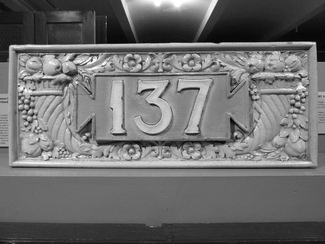
\includegraphics{sign.png}

Old Subway Station Sign, New York Transit Museum \\
New York City \\
{\tt http://kula.tproa.net/photos/2011/07/20110720-nyctrip/ }
\end{center}



\newpage

\thispagestyle{empty}
\vspace*{12cm}
\begin{sideways}
\Large{St. Joshua Norton Press}
\end{sideways}
\begin{sideways}
\Large{PO Box 980461}
\end{sideways}
\begin{sideways}
\Large{Ypsilanti MI 48198}
\end{sideways}


\end{document}


